%%% =============================================================
%\chapter*{Résumé en Français \texorpdfstring{\hfill\raisebox{-1em}{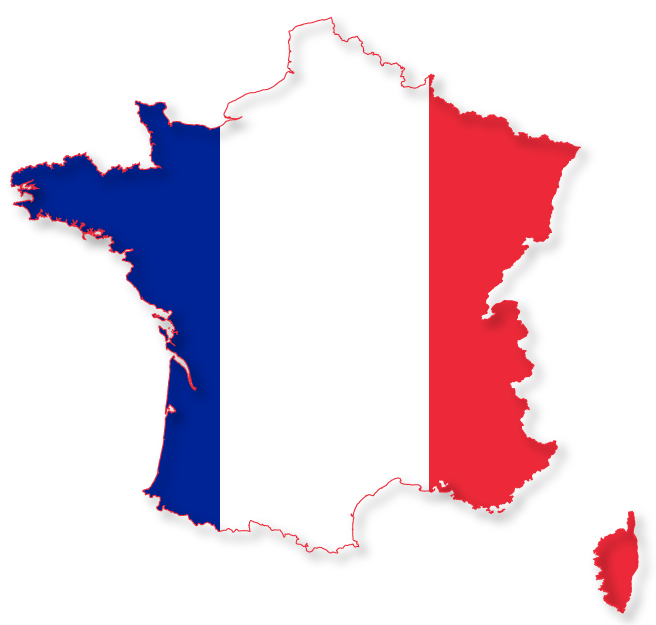
\includegraphics[height=2em]{img/france.png}}}{}}
%\addcontentsline{toc}{section}{\texorpdfstring{\protect\raisebox{-0.5ex}{\protect\makebox[3ex]{\protect
\includegraphics[height=1em]{img/flag-france.png}}}}{} in French}
%%% =============================================================
%%\index{Summary!en français}
%%\index{Summary!en français \protect\makebox[3ex]{\protect
\includegraphics[height=1em]{img/flag-france.png}}}
%\index{Summary!Résumé \protect\makebox[3ex]{\protect
\includegraphics[height=1em]{img/flag-france.png}}}
%
%Pour vous simplifier beaucoup de tâches longues et ardues, vous avez
%certainement déjà utilisé un ordinateur et en étiez très satisfaits.
%% 
%Cependant, de temps à autre, l'ordinateur ne fait pas ce que vous lui
%demandez: vous cliquez sur le bouton ``Faire ça'' et il ne le fait
%pas. Ou pire, l'ordinateur se bloque et ne répond plus à aucune
%commande. D'importantes heures de travail viennent peut-être de
%s'envoler.
%% 
%Vous gardez votre sang-froid, redémarrer l'ordinateur et tout semble à
%nouveau marcher comme prévu.
%% 
%L'erreur ne vient visiblement pas de l'ordinateur lui-même, mais elle
%semble venir du \emph{logiciel} qui contrôle ce dernier.
%% 
%Vous vous demandez pourquoi cette erreur n'a pas été corrigée, et qui
%plus est, pourquoi on ne s'est pas \emph{assuré} dès le départ que
%l'erreur ne survient pas. %survient
%
%Les différentes composantes électriques de la machine peuvent tomber
%en panne. Historiquement, ces erreurs sont appelées des \emph{bugs} %
%-- le terme anglais pour cafards -- %,
%car il est dit qu'un vrai cafard est entré un soir dans le châssis
%d'une machine qu'un informaticien fabriquait dans son garage,
%détruisant au passage quelques morceaux du circuit électrique. En se
%réveillant le lendemain, il s'est rendu compte que la machine
%manifestait un comportement bizarre.  Le terme est resté et est
%maintenant utilisé pour qualifier toutes sortes d'erreurs de
%programmation en général.
%% , c'est-à-dire quand un programme ne
%% solutionne pas le problème donné.
%
%Étant donné la complexité des ordinateurs de nos jours, il n'est pas
%étonnant qu'ils soient sujets à de nombreuses erreurs.
%% 
%Ils nécessitent de prendre en charge une multitude de
%paramètres, %et de caractéristiques,
%sans oublier les erreurs humaines introduites lors de la phase de
%programmation.
%% 
%C'est pourquoi %il est préférable
%la tendance est %
%de construire ces machines en composant plusieurs unités plus
%réduites.
%% 
%Chaque unité est de ce fait plus facile à contrôler, mais
%ces unités peuvent communiquer les unes avec les autres à n'importe
%quel moment.
%% 
%Il devient alors très difficile de prendre en compte tous les
%scénarios possibles et de prédire le comportement général du
%programme, à cause de ce caractère imprévisible. % hasardeux
%
%Les entreprises fabriquant ces logiciels n'ont pas intérêt à y laisser
%des bugs, puisqu'une erreur %quelque part
%peut engendrer d'autres erreurs en cascade.
%% 
%Celles-ci passent du temps, et de l'argent, à traquer ces bugs et s'il
%y en a trop, il n'est simplement plus rentable ou même envisageable de
%les éliminer.
%% 
%Les entreprises mettent donc en place, dans le cycle de développement de
%chaque projet, une phase essentielle de contrôle de qualité.
%% 
%Cela dit, certains bugs sont plus urgents à résoudre que d'autres.
%% 
%Ce n'est pas très grave si on ne peut pas décrocher son téléphone lors
%d'un appel, ou si l'éditeur de texte perd les derniers ajouts à notre
%document. C'est peut-être très ennuyeux mais le pronostic vital n'est
%pas engagé! On s'en remettra, en attendant la mise à jour du logiciel
%incriminé.
%% 
%Par contre, ce n
%'est pas le cas pour ces systèmes, dits
%\emph{critiques}, pour lesquels la sûreté est primordiale. Toutes les
%erreurs doivent être éliminées, qu'elles soient au niveau logiciel ou
%au niveau de la machine.
%% 
%Il n'est pas acceptable, par exemple, qu'un pacemaker s'arrête de
%fonctionner quand on passe le portique dans le métro, que l'avion
%parte en chute libre quand l'équipage allume le signal d'interdiction
%de fumer à bord, ou encore que deux trains entrent en collision parce
%que les feux ont mal fonctionné.
%% 
%% C'est pourquoi 
%Il est nécessaire de concevoir des techniques pour détecter ce genre
%d'erreurs.
%
%Pour améliorer la qualité des logiciels, il existe une technique
%prédominante: la méthode qui vise à soumettre le programme à une série
%de \emph{tests} et d'en observer les résultats.
%% 
%Ces scénarios de tests sont soigneusement conçus afin de couvrir un
%maximum d'exécution possible du programme.
%% 
%Dans la même catégorie, il est possible d'extraire un \emph{modèle} du
%programme %
%% , en prenant soin d'éliminer les morceaux superflus pour les
%% tests en cours, et 
%et de l'utiliser pour \emph{simuler} le programme.
%% 
%Cela dit, lorsque le programme est de plus en plus grand et complexe,
%que l'on utilise un modèle ou le programme lui-même, il devient
%impossible de \emph{garantir} que toutes les exécutions soient prises
%en compte par une batterie de scénarios.
%% 
%C'est même tout bonnement impossible lorsque le programme contient un
%paramètre qui varie sur un domaine non borné, comme par exemple, un
%entier.
%% 
%Ces deux méthodes sont utiles pour découvrir rapidement de simples
%erreurs, mais les erreurs subtiles, comme celles concernant le timing,
%restent non détectées.
%% 
%Dans le cas des systèmes qui requièrent une sûreté maxi\-male, il
%n'est pas concevable d'utiliser un programme qui pourrait contenir une
%erreur, quand bien même il ait passé tous ses tests.
%
%Comment donc s'assurer que toutes les exécutions d'un programme aient
%été prises en compte?
%% 
%On ne peut certainement pas faire tourner le programme et se contenter
%d'un ensemble restreint d'exécutions ou de valeurs pour les paramètres
%du programme.
%% 
%La technique d'\emph{analyse statique} offre une couverture complète
%d'un programme, sans l'exécuter. Elle inspecte toutes les exécutions
%\emph{faisables}, c'est-à-dire celles que le programme \emph{peut}
%effectuer et non celles qu'il \emph{va} effectuer.
%% 
%Le code source du programme y est sous la loupe, qu'il soit lisible
%par un humain ou seulement par une machine.
%% 
%Chaque combinaison est prise en compte ce qui rend cette méthode
%rapidement ingérable.
%% On pourrait être moins naïf, et se limiter à
%% certaines parties du code qui peuvent contenir les erreurs. Cependant,
%% déterminer leur emplacement est certainement aussi difficile que de
%% chercher les erreurs elles-même.
%% 
%% Il nous faut une autre méthode. %
%Cette thèse se concentre autour du problème suivant: %
%concevoir une méthode qui \emph{garantisse} qu'aucune erreur ne reste
%inaperçue, tout en restant dans des proportions raisonables.
%
%%% ------------------------
%Pour pouvoir vérifier qu'un programme soit correct, il s'agit d'abord
%de définir ce à quoi il doit se conformer ---appelé formellement sa
%\emph{spécification}.
%% 
%En listant l'ensemble des configurations à éviter, en listant tous les
%comportements souhaitables (ou une combinaison des deux), on décrit
%les propriétés que le programme doit satisfaire.
%% 
%Il en existe deux catégories: les propriétés de \emph{sûreté} et les
%propriétés de \emph{vivacité} (Safety et Liveness en anglais).
%% 
%Par exemple, ``le pacemaker ne s'arrête jamais'', ``l'airbag ne doit
%pas prendre plus de $x$~millisecondes pour s'ouvrir'', ou encore
%``aucun processus ne peut bloquer tous les autres'' sont des
%propriétés de sûreté. On doit s'assurer que le programme ne soit
%jamais dans une mauvaise configuration.
%% 
%À l'inverse, ``le facteur livre le courrier à son destinataire'', ``le
%système ne stagne pas'' ou encore ``le serveur prend en charge une
%requête internet'' sont des propriétés de vivacité, où l'on
%s'intéresse aux bonnes configurations du programme, associées à
%certaines probabilités.
%% 
%C'est à nous de définir ce que la spécification doit inclure, pour
%s'accorder avec la vérification souhaitée.
%% 
%Un système d'anti-blocage de freins (ABS), par exemple, calcule le
%freinage adéquate. Toutefois, si ce calcul ne se fait pas dans le
%temps imparti, le système n'est pas considéré comme un comportement
%désirable, et est donc défectueux.
%% 
%Dans cette thèse, nous nous concentrons sur les propriétés de sûreté.
%\begin{statement}
%  {\bf Sûreté}: %
%  {\it Étant donnée une spécification, le système peut-il se retrouver\\dans une mauvaise configuration?}
%\end{statement}
%
%%% ------------------------
%Plutôt que de tester le programme dans des scénarios particuliers, ou
%d'en analyser le code source, on utilise un cadre mathématique, dit de
%\emph{vérification formelle}, qui permette de \emph{prouver} qu'un
%programme soit conforme à sa spécification.
%% 
%Plus particulièrement, on cherche à prouver l'absence d'erreur, de
%manière \emph{automatique}, c'est-à-dire sans intervention de
%l'utilisateur.
%% 
%On commence par extraire un modèle qui corresponde aux comportements
%du programme origi\-nel, tout en en éliminant les parties sans
%rapport %importance
%au vu de la propriété à vérifier.
%% 
%Toutefois, comment faire lorsque le programme manipule des entités non
%bornées? On parle alors de système à états infinis et on en construit
%une approximation qui respecte malgré tout l'essence même du programme.
%
%De nombreux systèmes à états infinis peuvent en fait être caractérisés
%par une famille de systèmes à états finis, avec un paramètre (ou plus)
%variant dans un domaine non borné.
%% 
%Pour chaque valeur du paramètre, le système est à états finis.
%% 
%Le paramètre peut par exemple être 
%% la taille d'une base de données,
%le nombre de processus associés à une session donnée d'un protocole, %
%le nombre de n\oe{}uds dans les mailles d'un réseau, %
%ou encore l'agencement des différentes composantes d'un programme (et
%implicitement comment elles communiquent entre elles).
%% 
%Les systèmes qui contiennent un paramètre \emph{a priori} inconnu
%doivent se comporter correctement quelle que soit la valeur du
%paramètre. Ils sont ainsi considérés comme des systèmes à états
%infinis, et on les appelle des systèmes paramétrés.
%%
%%% ---------------------------
%Dans cette thèse, nous présentons deux méthodes pour vérifier certaines
%propriétés de sûreté de ces systèmes paramétrés.
% 
%La première méthode fait machine arrière: elle part des états erronés
%du système en général, et calcule à quoi ressembleraient les états du
%système qui pourraient mener à une erreur.
%% 
%Autrement dit, elle trouve l'ensemble des configurations qui sont
%directement et indirectement mauvaises.
%% 
%Si les états initiaux du système originel ne font pas partie de cet
%ensemble, le programme peut être considéré comme correct. Il faut bien
%sûr d'abord s'assurer que l'approximation du modèle extraite du
%programme de départ corresponde à ce dernier.
%
%La deuxième méthode démarre des états initiaux. Elle se limite à de
%petites valeurs du paramètre, et en déduit un seuil pour lequel il
%n'est pas nécessaire de continuer les calculs: la méthode a en effet
%toutes les données nécessaires pour conclure qu'il n'existe pas de
%mauvaises configurations pour les valeurs du paramètre plus grandes
%que ce seuil.
%% 
%En simplifiant, la méthode décompose chaque configuration en petits
%morceaux d'une certaine taille, et se charge de recombiner ces
%morceaux de toutes les manières possibles, en particulier en
%configurations de toutes tailles (un peu comme des briques de Lego).
%%
%L'idée est de collecter tous les petits morceaux, et de s'assurer
%qu'aucune des recombinaisons ne correspond à une mauvaise
%configuration.
%%
%Si c'est le cas, le seuil est trouvé. Si ce n'est pas le cas, on
%recommence avec des morceaux de taille un peu plus grande.
%
%En dernier lieu, il est intéressant de se demander dans quelles
%conditions la méthode termine. Le problème est classé dans la catégorie
%des problèmes indécidables, c'est-à-dire qu'il n'y a pas de méthode
%générale pour solutionner \emph{toutes} les instances du
%problème. Cela dit, pour certaines instances, ces deux méthodes
%s'avèrent être efficaces et peuvent même parfois être garanties de
%terminer.
%% 
%En effet, alors que d'autres méthodes prenaient des heures, ces
%méthodes permettent de vérifier certains programmes en quelques
%secondes, ce qui %Ces temps de calculs raisonnables étaient
%était le but recherché.
%%
%Cette thèse démontre notamment l'efficacité de ces méthodes en
%s'attaquant au problème complèxe d'analyse de formes, c'est-à-dire aux
%programmes concurrents manipulant des listes liées. %en mémoire.
%% \qed
